\documentclass{article}

\usepackage{../preamble}
\standalonetrue

\pagestyle{fancy}
\fancyhf{}
\rhead{Section \thesection}
\lhead{PHYS 304 Lecture 13}
\rfoot{Page \thepage}


\title{PHYS 304 Lecture 13}
\author{Ashtan Mistal}
\date{!!!}

\begin{document}

\ifstandalone
\maketitle
\fi

\graphicspath{{./Lecture13/}}

\section{Key points from last lecture}

We asked the question, what different operator, call it $\hat{W}$, would one have to operate on ket $\ket{\vec{r}'}$ with, such that with another ket $\ket{\vec{r}}$ is projected onto that modified ket $\hat{W} \ket{\vec{r}'}$, you get the same inner product when you operate on $\ket{\vec{r}}$ with $\hat{R}$, before projecting onto $\ket{\vec{r}'}$. i.e., for what operator $\hat{W}$ is $\bra{\vec{r}'} \left( \hat{R} \ket{\vec{r}} \right)$ equal to $\braket{ \left( \hat{W} \ket{\vec{r}'} \right) | \vec{r}}$?

We showed that $\braket{ \left( \hat{W} \ket{\vec{r}'} \right) | \vec{r}} = \braket{\vec{r}'|\hat{W}^+|\vec{r}}$, where the superscript $^+$ represents the complex conjugate of the transpose (the \textbf{adjoint}) of the operator, so that $\hat{W}$ must equal $\hat{R}^+$.

i.e. $\bra{\vec{r}'} \left( \hat{R} \ket{\vec r} \right) = \braket{ \left( \hat{R}^+ \ket{\vec{r}'} \right) \vec{r}}$ because $\bra{(\hat{R}^+ \ket{\vec{r}'}} = \bra{\vec{r}'}\hat{R}$

Check out the 2D graph from last day. 

\subsection*{2D real vector space sanity check: $\hat{R}(\theta)$}

$$\hat{R} (\theta)^+ = \hat{R} (\theta)^T = \hat{R}(- \theta)$$


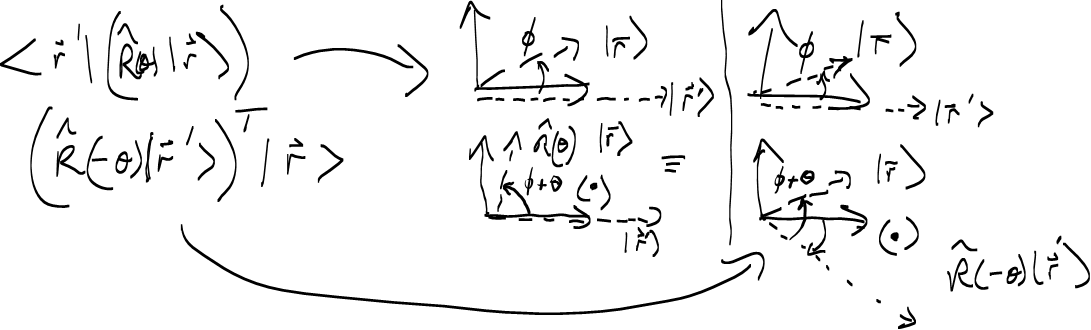
\includegraphics[width = 0.9 \textwidth]{Lecture13/1.png}

This also applies to differential operators:

$$\braket{f(x) | \frac{d}{dx} | g(x)} = \bra{f(x)} \left( \frac{d}{dx} \ket{g(x)} \right) = \braket{- \frac{d}{dx} f(x) | g(x)}$$

$$\Rightarrow \left( \frac{d}{dx} \right)^+ = \left( - \frac{d}{dx} \right)$$

NOTE: this is a direct analogy to the 2D vector space example, if we think in terms of matrix representations, but we also add the need to take the complex conjugate when evaluating the inner product; not just the transpose of the vector that is being projected from the left. 

i.e. $\braket{\vec{r}'|\vec{r}} = \begin{bmatrix} x'^* & y'^* \end{bmatrix} \begin{bmatrix} x\\ y \end{bmatrix}$

We also derived some properties of Hermitian operators ($\hat{O}^+ = \hat{O}$), based entirely on assumed eigen "states" and corresponding eigen values of that operator, in abstract "state space":

$$\hat{O} \ket{O} = \hat{O}^+ \ket{O} = O \ket{O}$$

\begin{itemize}
    \item Operators with real expectation values for any arbitrary state must be Hermitian
    \item eigen states that have zero variance in their expectation values for Hermitian operators must be eigen states of those Hermitian operators
    \item When the eigen spectrum is discrete for such Hermitian operators, then the eigen values must be real, the eigen states corresponding to different eigen values are orthogonal, and a complete orthonormal basis that spans the relevant “state space” can be formed from them.
\end{itemize}

\section{Immutability of quantum mechanical states and Hilbert space}


\begin{itemize}
    \item Reinforce the immutable nature of quantum mechanical “states” and operators that exist in a system’s Hilbert space
    \item Put what we have done so far in the course, all in terms of differential operators in 1 dimensional x space, in this larger context of abstract Hilbert space
\end{itemize}

\subsection{Activity 1}

What are 3 ways you already know of how to specify $\Psi(x,t)$ at some specific time $t$, say, $t = 0$?

$$\Psi(x,0) = f(x), \quad \Psi(x,0) = \sum_n c_n \psi_n(x)$$

$$f(x) = \frac{1}{\sqrt{2 \pi}} \int F(k) e^{ikx} dk = \Psi(x,0)$$

$$\left\{ c_n \right\}, \quad \left\{ f(x) \right\}, \quad \left\{ F(k) \right\}, ...$$


Recall we discussed previously that you can expand $\psi(x,t=0)$ in terms of the stationary eigen states of the total energy operator, $\psi_n$, which we were told form a complete orthonormal set of functions, that can be used to expand/represent any square integrable function in x, with the inner-product defined as $\int (\psi_n*(x) f(x) dx$.   Previously you have been told that you can expand an arbitrary square integrable function in terms of a Fourier series or Fourier transform, with the same inner product rule, where there $\psi_n(x)=e^(-ikx)$.  So this is sort of like having different bases, $\ket{\hat{\alpha}_1}$  and $\ket{\hat{\alpha}_1}$, in 2D real vector space. 

\hfill

Thus there must be some immutable state that represents the essence of a quantum mechanical particle’s temporal evolution, subject to some potential.  That state can be fully described using any number of expansions in distinct bases that each span the more general Hilbert state space of the problem. 

Let an arbitrary quantum state be designated by $\ket{S(t)}$. 

Write a general expansion for the expansion of $\ket{S(t)}$ in an arbitrary basis $\left\{ \ket{O_n} \right\}$ defined by some Hermitian operator. Draw an analogy with the 2D real vector space examples. 

$$\ket{S(t)} = \sum_n \braket{O_n | S(t)} \ket{O_n} = \left( \sum_n \ket{O_n} \bra{O_n} \right) \ket{S(t)}$$

SO, the set of basis vectors look very similar to the $\ket{\hat{\alpha}_1}$ and $\ket{\hat{\alpha}_2}$ from the 2D vector example. 

More importantly, where did the $x$ go? Where are the wavefunctions?

What would you choose to define the state at time $t$? ($c_n$ in $H$ basis, $\Psi(x,0)$?, $\Phi(k,0)$, or in some \textbf{other} observable's eigen states? (point is, you can choose any of them, so generally can keep equations general, in Dirac notation, without specifying a particular representation, until you start actually solving a specific problem, at which there may be a "natural representation" to choose. Often, when we get down to the nitty gritty, we end up using $\Psi(x,0)$ in analogy to $\hat{i}$, $\hat{j}$. 

\subsection{Activity 2}


In 2D real vector space, we learned all the manipulations in the $\ket{\hat{i}}$ and $\ket{\hat{j}}$ basis,.before introducing other, more general orthonormal bases, $\ket{\hat{\alpha}_1}$ and $\ket{\hat{\alpha}_2}$. 

IN quantum mechanics, we learned how to do crucial calculations using wavefunctions $\Psi(x,t)$, that involve differential operators and differential equations that act on functions that are part of the Hilbert space defined by square integrable equations in position space. At any given time $t$, the complex wavefunction is a function of$x$,  that specifies a complex \textit{amplitude} of $\Psi(x,t)$ at \textit{every point} $x$. 

\hfill

What is the relationship between $\Psi(x,t)$ and $\ket{S(t)}$?

$$\ket{S(t)} = \sum_n \ket{O_n} \bra{O_n} | S(t)$$

Let $\ket{O_n} \rightarrow \ket{x_n} \rightarrow \ket{x}$

$$\Longrightarrow \ket{S(t)} = \int_{- \infty}^\infty dx \ket{x} \bra{x} \ket{S(t)} = \int_{- \infty}^\infty \braket{x|S(t)} \ket{x} dx$$

Compare with $\Psi(x,t) = \sum_n c_n \Psi_n(x,t) = \sum_n \int_{- \infty}^\infty \Psi_n^*(x') \Psi(x',t) dx' \Psi_n(x)$

where $\psi_n(x)$ are eigenfunctions of the total energy operator in 1D $x$-space.

$\ket{x}$ are the eigen \textbf{states} of the position operator in abstract Hilbert space, whereas $\psi_n(x)$ are the eigen \textbf{functions} in the total energy operator in 1D $x$-space. 

$\braket{x|S(t)}$ is the projection of the abstract state at time t in Hilbert space onto the eigen states of the position operator in abstract Hilbert space; $\int_{- \infty}^\infty \psi_n^*(x') \Psi(x',t) dx'$ is the projection of the full wavefunction in 1D x-space onto the eigen functions of the total energy operator. 

Therefore, $\Psi(x,t) = \braket{x|S(t)}$

i.e. our wavefunction is merely the projection of the immutable state of the particle at any time $t$, onto eigenstates of the immutable position operator with eigenvalues $x$!


\subsection{Activity 3}

The equivalent of our “standard”, or “inertial” basis in 2D real vector space, $\hat{i}$ and $\hat{j}$, in the case of Hilbert Spaces in Quantum Mechanics, is the position basis, which in 1D, as we have dealt with exclusively to this point, is simply the space spanned by $x$.  

Lets better understand the nature of “the position basis”.  What defines it?


Note that in the 2D vector space example, to do any actual calculations, (e.g. the projection of an arbitrary state onto an arbitrary alpha basis state), in practice you end up writing all the states in terms of the inertial reference frame, and then going the dot product. In quantum mechanics, it is fairly similar, and the usual / traditional "inertial" reference frame / basis are $\{\ket{r}\}$. 

\subsubsection*{Activity Questions}

$\hat{x} \ket{x} = x \ket{x}$ for a continuous space. What are $\hat{x}, x, $and $\ket{x}$?

\hfill

What is the wavefunction of a position operator's eigen state?

If $\braket{x'|S(t)} = \Psi_{\ket{S}} (x',t)$, and if $\hat{x} \ket{x} = x \ket{x}$, then we have the following:

$$\Psi_{\ket{x}} (x') = \braket{x'|x} = \delta(x - x')$$

Thus, in the position basis, we have the following:

$$\ket{S(t)} = \int_{- \infty}^\infty \ket{x} \bra{x} \ket{S(t)} dx$$

$$\ket{S(t)} = \int_{- \infty}^\infty \braket{x|S(t)} \ket{x} dx$$

$$\Longrightarrow \braket{x'|S(t)} = \Psi_{\ket{S(t)}} (x',t) = \int_{- \infty}^\infty \Psi_{\ket{S(t)}} (x,t) \braket{x'|x} dx$$

$$\Psi_{\ket{S(t)}} (x',t) = \int_{- \infty}^\infty \Psi_{\ket{S(t)}} (x,t) \Psi_{\ket{x}} (x') dx = \int_{- \infty}^\infty \Psi_{\ket{S(t)}} (x,t) \delta(x - x')$$

Therefore must think of our $\Psi(x,t)$ as merely a list of (complex) projections of the more general, immutable, abstract state of the particle, $\ket{S(t)}$ onto each abstract eigen state of the immutable $\hat{x}$  operator with (real) eigen values $x$.


$$\begin{matrix}
& & \text{Need to specify:} \\
\Psi(x,0) = \sum_n c_n \psi_n(x) & \longrightarrow &  \{c_n\} \{ \psi_n(x)\} \\
\hfill
= \frac{1}{\sqrt{2 \pi}} \int_{- \infty}^\infty dk F(k) e^{ikx} & \longrightarrow & \{F(k)\} \{e^{ikx}\} \\
\hfill
= f(x) & \longrightarrow & \{f(x)\} \{\delta(x-x')\}; \int \text{is trivial}
\end{matrix}$$



\end{document}